\documentclass[a4paper, 10pt, twocolumn]{article}

% Configuration {{{
\usepackage[utf8]{inputenc}
\usepackage[T2A]{fontenc}
\usepackage[english, russian]{babel}

\usepackage{enumitem}
\setlist{nolistsep}
\usepackage{mathtools}
\usepackage{xcolor}
\definecolor{dimblue}{HTML}{1010aa}
\usepackage[
	colorlinks=true, 
	allcolors=dimblue
]{hyperref}
\usepackage[
	vmargin=1in,
	hmargin=.8in
]{geometry}
\setlength{\columnsep}{.25in}
%\usepackage[nospread]{flushend}
\usepackage{cuted}
\linespread{1.3}
\usepackage{indentfirst}
\usepackage{graphicx}
\usepackage[multidot]{grffile}
\usepackage[labelsep=period]{caption}
\usepackage{subcaption}

\usepackage{titlesec}
\titleformat{\section}[hang]{\bf\centering}{\thesection.}{.5em}{}[]
\def\thesection{\Roman{section}}
\def\thefootnote{\fnsymbol{footnote}}

\usepackage{ifthen}
\newboolean{articletitles}
\setboolean{articletitles}{true}
\newboolean{italicNames}
\setboolean{italicNames}{false}
\newboolean{italicTitles}
\setboolean{italicTitles}{true}
% }}}


\begin{document}

% Title {{{
\begin{strip}
\begin{center}
\vskip-2.4\baselineskip
{\bf\large Модели суперсимметрии. Поиск суперсимметрии на БАК}
\vskip.3\baselineskip
{Керим Гусейнов\footnotemark}
\vskip.3\baselineskip
\today
\end{center}
\end{strip}
\footnotetext{\href{mailto:guseynovkerim@gmail.com}{guseynovkerim@gmail.com}}
% }}}

\section{Введение}
% {{{

В физике частиц Стандартная модель на данный момент является 
самой успешной и с большой точностью описывает многие процессы 
и реакции. Однако существуют глобальные явления, объяснить 
которые в рамках СМ все еще не удается. Список таких явлений 
включает
\begin{itemize}
	\item осцилляции нейтрино;
	\item барионную асимметрию вселенной;
	\item темную материю;
	\item стабильность массы бозона Хиггса из-за петлевых поправок;
	\item иерархию масс фундаментальных частиц.
\end{itemize}
Кроме того, СМ не притрагивается к объяснению гравитации и даже 
несовместима с наиболее успешной из существующих моделей ее -- общей 
теорией относительности.

Поскольку СМ согласуется с экспериментом с большой точностью и любые 
новые теории обязаны описывать прошедшие эксперименты с не меньшей 
точностью, можно искать новые теории в виде расширения Стандартной 
модели. Существует множество способов сделать это, самые популярные из 
которых -- теории великого объединения и суперсимметрии. Суперсимметрия 
имеет пространственно-временной характер и предполагает симметрию 
относительно бозонов и фермионов, то есть существование 
суперсимметричного партнера бозона для каждого фермиона и наоборот. 
В идеальном случае, когда суперсимметрия не нарушена, массы и все 
остальные внутренние квантовые числа партнеров, за исключением спина, 
совпадают. В частности, это приводит к тому, что положительное 
вакуумное среднее бозонов и отрицательное фермионов полностью друг 
друга компенсируют, оставляя в итоге строгий ноль. Однако до сих пор, 
несмотря на все усилия, не было найдено экспериментальных свидетельств 
существования суперсимметрии, то есть если она вообще существует, то 
значительно нарушена. Тем не менее все еще существует большая тяга 
к теориям суперсимметрии, обусловленная тем, что в конечном итоге они 
позволяют включить гравитацию в квантовый подход и, более того, они 
подкреплены теорией струн.

% }}}

\section{Частицы суперсимметричных моделей}
% {{{

Суперсимметрия может быть введена различными способами. Наименьшим 
образом изменяет Стандартную модель так называемая Минимальная 
суперсимметричная стандартная модель (МССМ). Поскольку ни одна частица 
СМ не может быть суперпартнером какой-либо другой в рамках СМ, 
количество частиц в МССМ должно как минимум удвоиться. Партнеров 
кварков называют скварками, лептонов -- слептонами, а глюонов, фотона, 
$W$ и $Z$ бозонов и гравитона -- глюино, фотино, вино, зино и гравитино 
соответственно. Кроме того, ввиду дополнительных требований к полю 
Хиггса, помимо уже открытого скалярного бозона Хиггса, необходимо также 
ввести один тяжелый скалярный, один псевдоскалярный и два заряженных 
бозона Хиггса~\cite{intro2005}. Электрически нейтральные суперпартнеры 
бозонов хиггсино, вино, а также отвечающий за слабый гиперзаряд бино 
перемешиваются и дают 4 состояния $\tilde{\chi}^0_1, ... 
\tilde{\chi}^0_4$, называемых нейтралино. Также смешивание частиц 
приводит к образованию двух заряженных состояний $\tilde{\chi}^\pm_1$, 
$\tilde{\chi}^\pm_2$, называемых чарджино. В основном они распадаются 
через $W^\pm$ и $Z$ бозоны на более легкие суперчастицы
$$ \tilde{\chi}^0_2 \to \tilde{\chi}^0_1 + Z,
\quad
\tilde{\chi}^0_2 \to \tilde{\chi}^\pm_1 + W^\mp, $$
$$ \tilde{\chi}^\pm_2 \to \tilde{\chi}^\pm_1 + Z,
\quad
\tilde{\chi}^\pm_1 \to \tilde{\chi}^0_1 + W^\pm. $$

В рамках суперсимметрии также вводится понятие $R$-четности, выражающее 
принадлежность частицы к обычным или к суперпартнерам, 
$R~=~\left(-1\right) ^ {3(B-L) + 2s}$. Важно заметить, что, аналогично 
теориям великого объединения, барионное и лептонные числа не могут 
сохраняться в рамках суперсимметрии~\cite{baryon-lepton-violation}, 
однако их разность сохраняется. $R$-четность всех частиц равна единице, 
а суперпартнеров -- минус единице.

$R$-четность, как и многие другие мультипликативные законы сохранения, 
нарушается или может быть потенциально нарушена. Существуют как теории 
суперсимметрии, в которых $R$-четность строго сохраняется, так и те, 
в которых нарушается. При сохранении $R$-четности суперпартнеры 
рождаются и существуют парами, в результате чего, если не аннигилируют, 
распадаются на более легких суперпартнеров. Таким распадам, очевидно, 
есть предел. Легчайшая суперчастица (ЛСЧ) должна быть стабильной. Кроме 
того, судя по тому, что мы все еще не наблюдали их в экспериментах, они 
слабо взаимодействуют с частицами СМ, а значит являются кандидатами на 
роль темной материи. В теоретических моделях в основном в качестве ЛСЧ 
выбирают нейтралино $\tilde{\chi}^0_1$, но также популярностью 
пользуется и гравитино $\tilde{G}$~\cite{models}. В последнем случае 
массовые параметры моделей часто выбираются так, чтобы более тяжелые 
чарджино и нейтралино почти всегда распадались в $\tilde{\chi}^0_1$, 
а сам $\tilde{\chi}^0_1$ распадался на $Z$ бозон и гравитино. В моделях 
без сохранения $R$-четности возможны распады $\tilde{\chi}^0_1$ на 
лептоны или кварки, что еще более усложняет ситуацию.

Помимо МССМ существует множество моделей суперсимметрии. В частности, 
модель, называемая следующей за минимальной суперсимметричной 
стандартной моделью (СМССМ), вводит дополнительное синглетное хиральное 
суперполе, чтобы решить проблему натуральности некоторых хиггсовских 
слагаемых лагранжиана МССМ. Однако вследствие этого в СМССМ появляется 
два новых бозона Хиггса, и хиггсовский сектор теряет $CP$ 
инвариантность. Помимо натуральности в МССМ присутствует еще одна 
проблема: число свободных параметров модели чрезвычайно велико. Если 
в СМ их было 19, и это уже рассматривалось недостатком, то в МССМ это 
число возрастает до 120. На МССМ можно наложить некоторые ограничения, 
закрепив значения одних параметров и связав между собой другие, и таким 
образом уменьшить число параметров. Разные ограничения, накладываемые 
на МССМ приводят, например, к ограниченной \mbox{МССМ} 
и к феноменологической МССМ.

Приведенный список моделей не является исчерпывающим. Некоторые другие 
модели различаются источниками нарушения суперсимметрии, наличием 
других дополнительных частиц и прочим.

% }}}

\section{Поиски суперсимметрии на БАК}
% {{{

Для обнаружения суперсимметричных частиц на коллайдерах необходимо 
определить характерные черты событий с их участием, а для этого более 
подробно рассмотреть их рождение и распады.

% ATLAS-CONF-2020-040 {{{

\begin{figure}[b!]% {{{
	\centering
	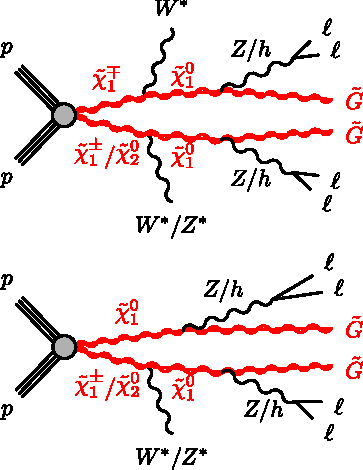
\includegraphics[width=.7\linewidth]{figures/4lepton-Feynman}
	\caption{Диаграммы Фейнмана рождения и распада легких нейтралино 
	и чарджино при ЛСЧ гравитино в модели с сохранением $R$-четности. 
	Сигнатура событий -- четыре лептона.}
	\label{fig:chi12-gravitino}
\end{figure}% }}}

Рассмотрим легкие нейтралино и чарджино в случае, когда ЛСЧ 
является гравитино. Их рождение и распад представлены на 
рисунке~\ref{fig:chi12-gravitino}. Промежуточные виртуальные $W$ и $Z$ 
дают слишком мягкие лептоны, не регистрируемые детектором. Таким 
образом, сигнатура событий с рождением легких чарджино и нейтралино при 
ЛСЧ гравитино -- 4 лептона. К тем же конечным состояниям приводят 
и некоторые процессы СМ: образование $ZZ$, $t\bar{t}Z$, трех 
электрослабых бозонов или Хиггса. Соответствующий анализ был проведен 
на основе 139 фб$^{-1}$ данных, собранных детектором ATLAS во время 
Run~II~\cite{ATLAS-CONF-2020-040}.

В анализе отбор событий производился несколькими способами, и для 
каждого из них на основе генераторов, очевидно, описывающих Стандартную 
модель, оценивались вклады за счет процессов СМ. Сравнение СМ 
и результатов эксперимента приведено на рисунке~\ref{fig:4l-events}. 
Как видно, числа событий в некоторых ячейках чрезвычайно малы, порядка 
5. Основные различия между данными и СМ прослеживаются именно в таких 
ячейках. При интерпретации результатов, кроме случая с сохранением 
$R$-четности, были также рассмотрены модели с её нарушением. В этом 
случае очередной проблемой является параметризация возможных распадов 
ЛСЧ. На основе результатов эксперимента можно составить пределы 
исключения масс ЛСЧ и частицы, следующей за ЛСЧ, они приведены на 
рисунке~\ref{fig:4l-limits}. Как видно, результаты существенно зависят 
от предположений, используемых в моделях. Тем не менее, допустимые 
массы суперсимметричных партнеров по мере появления новых анализов 
оказываются все больше и больше.

\begin{figure}[p]% {{{
	\centering
	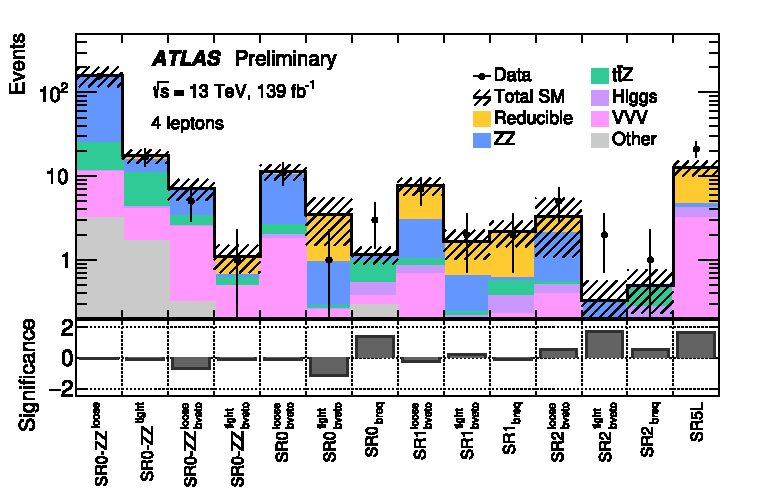
\includegraphics[width=\linewidth]{figures/4lepton-events}
	\caption{Ожидаемые и наблюдаемые количества событий для различных 
	способов отбора.}
	\label{fig:4l-events}
\end{figure}% }}}

\begin{figure}[p]% {{{
	\centering
	\begin{subfigure}{.9\linewidth}
		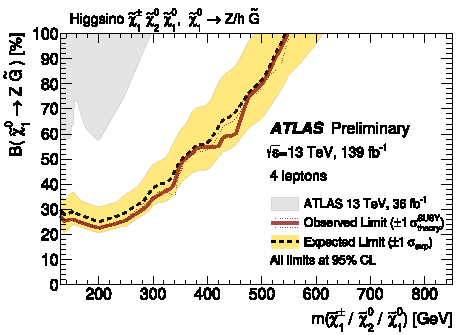
\includegraphics[width=\linewidth]{figures/4lepton-limits-higgsino}
		\caption{}
		\label{fig:4l-limits:higgsino}
	\end{subfigure}
	\begin{subfigure}{.9\linewidth}
		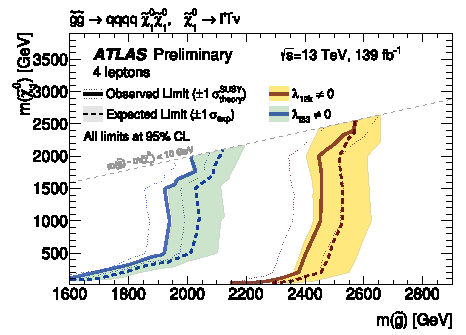
\includegraphics[width=\linewidth]{figures/4lepton-limits-gluino}
		\caption{}
		\label{fig:4l-limits:gluino}
	\end{subfigure}
	\caption{Ожидаемые (пунктирные) и наблюденные (сплошные) границы масс 
	частиц и вероятностей каналов в случае с сохранением~(a) 
	и нарушением~(b) $R$-четности.}
	\label{fig:4l-limits}
\end{figure}% }}}

% }}}

% ATLAS-CONF-2020-047 {{{
Еще один анализ был проведен на основе того же набора 
данных~\cite{ATLAS-CONF-2020-047}. В нем уже рассматривались лишь 
модели с сохранением $R$-четности, в рамках которых суперпартнеры 
рождаются парами, и поэтому велся поиск образования пар счастиц: глюино 
или скварков. Глюино и скварки рождаются из протонов в сильном 
взаимодействии, а инвариантная масса 13 ТэВ должна предоставить 
чувствительность к суперчастицам с массами порядка нескольких ТэВ. 
В рассматриваемых моделях глюино распадаются на легкие чарджино и два 
легких кварка, а скварки распадаются на те же чарджино, но один легкий 
кварк. Чарджино затем испускает $W$\babelhyphen{nobreak}бозон 
и образует легчайшее нейтралино. Соответствующие диаграммы Фейнмана 
представлены на рисунке~\ref{fig:gg-qq}. Частицы, не появляющиеся 
в цепях распадов явным образом, считаются находящимися вне 
кинематического доступа. Кроме того, вероятность всех участвующих 
в рассмотрении распадов считается равной 100\%. В эксперименте 
описанные события искались по наличию изолированного лептона от распада 
$W$, хотя бы двух струй и большой недостающей поперечной энергии от 
нейтрино и нейтралино. К аналогичному конечному состоянию приводят 
также некоторые процессы СМ: образование $t\bar{t}$-пар, единичных 
топ\babelhyphen{nobreak}кварков или $tW$, векторных бозонов со струями, 
$t\bar{t}$-пар в комбинации с векторным бозоном, а также образование 
пары векторных бозонов.

\begin{figure}% {{{
	\centering
	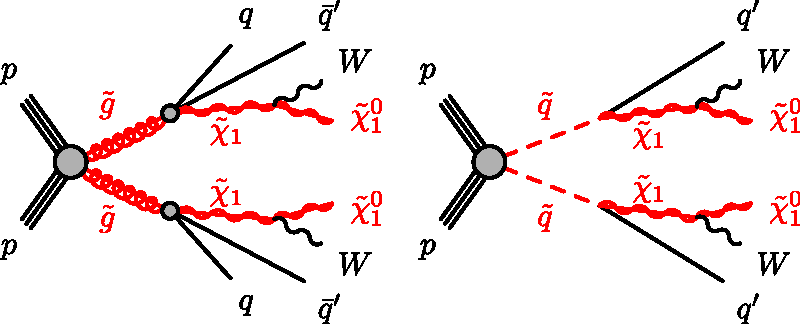
\includegraphics[width=\linewidth]{figures/gg-qq-Feynman}
	\caption{Диаграммы Фейнмана рождения и распада пар глюино (слева) 
	и скварков (справа) при ЛСЧ нейтралино и сохранении $R$-четности.}
	\label{fig:gg-qq}
\end{figure}% }}}

В анализе события разделялись на группы с разным количеством струй, 
с наличием или отсутствием струй от $b$\babelhyphen{nobreak}кварков, 
а также по величине эффективной массы, являющейся скалярной суммой 
поперечных импульсов лептона и струй и недостающей поперечной энергии. 
Сравнение чисел событий, определенных из эксперимента и вычисленных на 
основе СМ, приведено на рисунке~\ref{fig:gg-qq-events}. Некоторые 
экспериментальные точки превосходят фон СМ, однако существенного 
избытка событий не наблюдается. Выдвигаемые ограничения на массы 
частиц зависят от свободных и фиксированных параметров модели, а также 
от выбора самой модели. Для случая, когда масса чарджино находится 
ровно между массами скварка (или глюино) и нейтралино, найденные 
пределы допустимых масс счастиц представлены на 
рисунке~\ref{fig:gg-qq-limits}.

\begin{figure}[p]% {{{
	\centering
	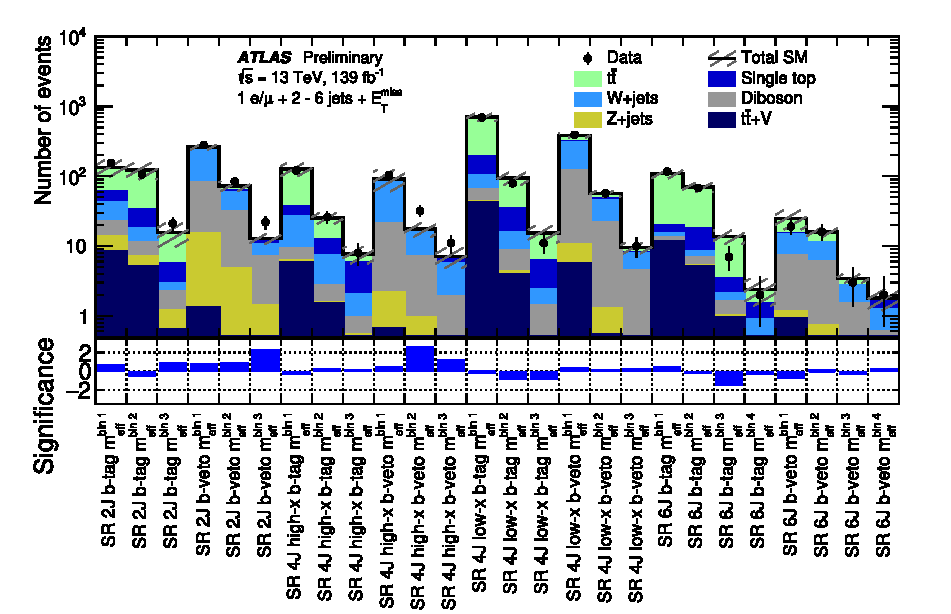
\includegraphics[width=\linewidth]{figures/gg-qq-events}
	\caption{Ожидаемые и наблюдаемые числа событий в различных группах 
	отбора.}
	\label{fig:gg-qq-events}
\end{figure}% }}}

\begin{figure}[p]% {{{
	\centering
	\begin{subfigure}{\linewidth}
		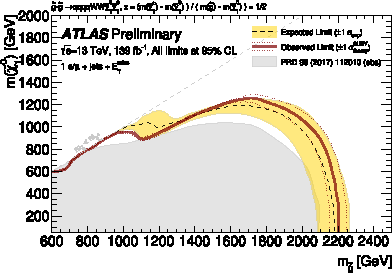
\includegraphics[width=\linewidth]{figures/gg-qq-limits-mg}
		\caption{}
		\label{fig:gmass-limit}
	\end{subfigure}
	\begin{subfigure}{\linewidth}
		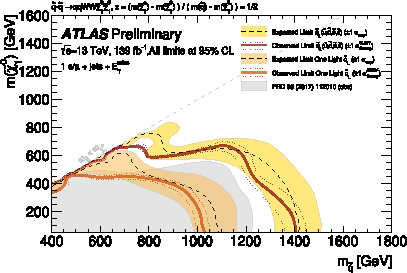
\includegraphics[width=\linewidth]{figures/gg-qq-limits-mq}
		\caption{}
		\label{fig:qmass-limit}
	\end{subfigure}
	\caption{Ожидаемые (пунктирные) и наблюденные (сплошные) пределы 
	допустимых масс глюино~(a) и скварка~(b) для упрощенной модели 
	суперсимметрии.}
	\label{fig:gg-qq-limits}
\end{figure}% }}}

Результат предыдущего анализа ATLAS, проведенного на меньшей статистике 
тремя годами ранее~\cite{gg-qq-earlyRun2}, давал пределы 2.1~ТэВ для 
глюино и 1.25~ТэВ для скварков. Увеличение статистики позволило 
расширить запрещенную зону до 2.2~ТэВ для глюино и 1.4~ТэВ для кварков.
% }}}

% }}}

\section{Вывод}
% {{{

С точки зрения теории, суперсимметрия чрезвычайно выгодна. Она 
позволяет решить многие вопросы, касающиеся вида лагранжиана. Она 
позволяет включить в рассмотрение гравитацию, прежде никогда не 
затрагивавшуюся. И кроме того, своими корнями она уходит в теорию 
струн. Многие нерешенные проблемы Стандартной модели даже не возникли 
бы в рамках суперсимметрии.

Со стороны эксперимента, однако, она не сыскала такого же успеха. 
Долгие годы исследований и многочисленные эксперименты дают лишь 
ограничения на значения параметров суперсимметричных моделей. Многие 
теоретики уже приняли это за опровержение суперсимметрии, но все еще 
остаются и сторонники, и их можно понять. Любые запреты на значения 
параметров выдвигаются относительно конкретной модели, причем обычно 
используются упрощенные. Полноценные модели суперсимметрии содержат 
настолько большое количество параметров, что, кажется, полностью 
отвергнуть их не будет возможно никогда. Хоть это и явно не сильная 
сторона теории, она позволяет ей все еще выживать.

В любом случае, суперсимметрия, очевидно, находится под большим 
давлением, а Стандартная модель нуждается в новых расширениях и новых 
возможностях проявления новой физики.

% }}}

\newpage
\bibliographystyle{local}
\bibliography{refs.bib}

\end{document}
% Trash {{{
Суперструны.

Смирнова
Ишханов Капитонов Юдин -- 447 499 503 504
Википедия русская, английская
\url{https://twiki.cern.ch/twiki/bin/view/LHCPhysics/SUSYCrossSections}


%%%%%%%%%%%%%%%%%%%%%%%%%%%%

\begin{itemize}
	\item Tell about different models, starting from the minimal.
	\item Tell about why we need all five Higgs bosons in SUSY.
	\item Tell about $CP$ violating stuff in the models beyond the SM.
	\item Look at slide 38, HEP-L8-Bphys.
\end{itemize}
%}}}
